\chapter{Incremental Dense Refinement}
\label{ch:incrDenseRef}
The reconstruction methods described thus far, build a manifold mesh from a set of sparse data. 
The outcome is able to capture the coarse geometry of the mesh, and even after the mesh sweeping, the reconstruction still lacks to capture the fine-grained details.
In this chapter we aim at recovering the details of the geometry of the scene, incrementally, by means of variational optimization which directly evolves the surface of the scene according to images. 
We present a fully automatic pipeline to incrementally estimate the accurate reconstruction. In particular the method described is able to handle multi-resolution mesh: instead of merging accurate submaps of the scene a-posteriori and off-line, it combines directly online the reconstruction refined with the variational algorithm together with the new rough manifold estimated with the algorithms presented in the previous chapters.

\minitoc

\section{Rationale}

Classical Multi-View Stereo methods \cite{gargallo2005bayesian,delaunoy_et_al_08} handle small objects, e.g., those proposed in the benchmark of Stretcha \etal \cite{strecha2006combined}.
The reasons are related both to the computational and memory resources needed to handle big set of images, and to the limitations of the optimization procedures.
The common volumetric voxel-based representation of the space requires a huge amount of memory to store accurate and detailed data.
Thanks to the introduction of hashing methods and especially  Delaunay Triangulation based methods, algorithms to deal with large-scales scenes have been proposed.
Successful Delaunay-based incremental approaches have been proposed in \cite{lovi_et_al_11,hoppe2013incremental,litvinov_lhuillier_13,romanoni15b,romanoni15a} but they all rely sparse data and visibility-only information, therefore the final reconstruction lacks in details and is not photo-consistent.


A very popular class of  incremental dense reconstruction algorithms relies on depth maps; they first estimate the depth map for a selected set of keyframe, then they merge the depth maps into a single consistent 3D model of the scene. 
Most of the depth maps-based approaches \cite{pollefeys_et_al_08,collins1996space,newcombe2010live,ohtake2003multi,stuhmer2012parallel,stuckler2014multi} rely on a voxel-based volumetric representation of the TSDF and are not suitable for large-scale reconstruction. 
Sch{\"o}ps \etal \cite{schops20153d} propose then to use voxel hashing together with a careful filtering of noisy depth data.
Even if the results are remarkable, the resulting model is a non-continuous mesh, and the meshing step is not directly driven by the images, but by marching cubes \cite{lorensen1987marching} that interpolates the TSDF , as in most of the depth map based approaches.

Mesh-based algorithms represent an effective alternative to depth-maps based reconstruction. Labatut \etal \cite{labatut2007efficient} estimate directly a visibility and photo-consistent mesh from the Delaunay triangulation of the 3D noisy points obtained from the depth maps.
Vu \etal  \cite{vu_et_al_2012} improve this algorithm by estimating an initial visibility-consistent mesh then by evolving the mesh such that it maximizes the photo-consistency with respect to the images. 
These Delaunay-based volumetric approaches are able to handle large scale scenes, but both \cite{labatut2007efficient} and \cite{vu_et_al_2012}  are not incremental.
Moreover, in the remarkable work of Vu \etal \cite{vu_et_al_2012}, the reconstruction pipeline   is not fully automatic, since the optimization method is well suited for 2-manifold meshes, but the method proposed to estimate the initial mesh does not guarantee that manifold property holds for the whole model.



In this chapter we propose a framework to overcome the previous limitation, which is the first incremental algorithm for large-scale environments, which reconstruct a continuous and photo-consistent manifold mesh. 
We propose a fully automatic pipeline that integrates existing works on manifold reconstruction with the accurate surface evolving refinement step and a novel manifold-preserving mesh merging algorithm.


\section{Proposed system}
 Our approach combines two parallel systems in order to provide a fully automatic and incremental reconstruction of the environment, which is photo-consistent with the images. In Fig. \ref{fig:architecture} we illustrate a scheme of the whole system.
 
 \begin{figure}[t]
  \centering
  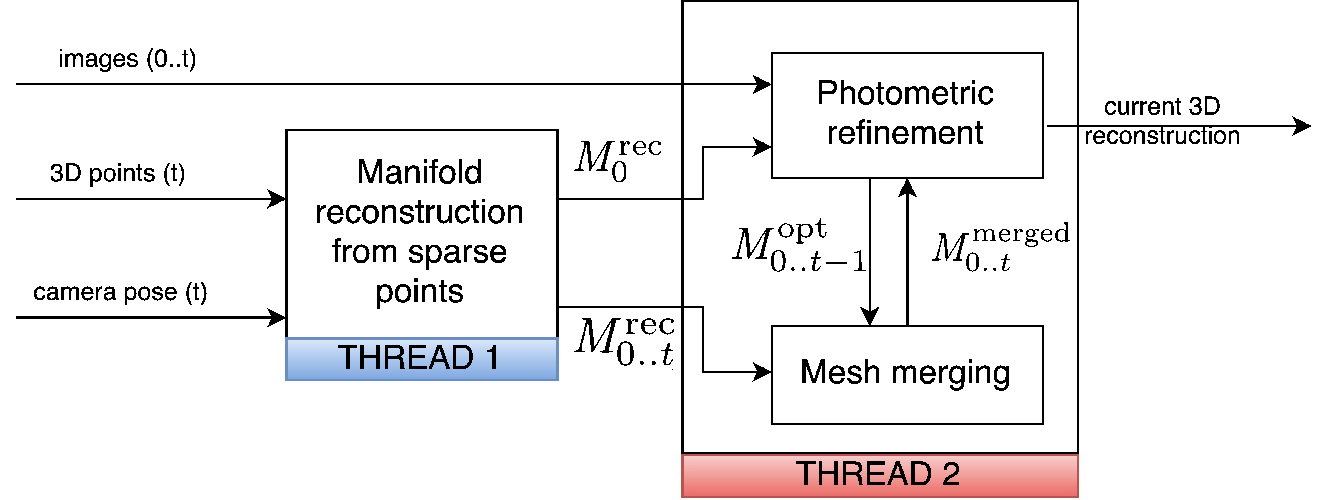
\includegraphics[width=\textwidth]{./img/ch-incr-dens/incremental-mvs-architecture}
  \caption{Architecture of the parallel and incremental reconstruction system}
  \label{fig:architecture}
\end{figure}


The proposed system runs two threads in parallel.
The first thread estimates the rough manifold mesh following the approach proposed in \cite{litvinov_lhuillier_13,romanoni15a}: it builds incrementally a manifold mesh bootstrapping from Structure from Motion 3D points and camera poses, this leads us to obtain a first fast initialization for the subsequent step. The output of this module is a mesh $\mathit{M}_{0..t}^{\text{rec}}$ that models the scene captured up to time $t$.

A second thread is dedicated to the windowed refinement of the mesh between images $t-W$ and $t$ and it adopts a variational approach to refine the mesh: it evolves the surface in order to maximize the photo-consistency between subsequent pairwise cameras. This approach reaches very accurate results and have been proved to scales well with large-scale scenes \cite{vu2011large}.
Moreover, we enforced the manifold property in the previous step in order to  consistently apply this mesh evolution process (see Section \ref{subsec:why}). 
The output of this module is the refined mesh $\mathit{M}_{0..t}^{\text{opt}}$ up to time $t$.
After the previous refinement, in the second thread we implemented a new approach to merge a new rough mesh generated at time $t$ by the first thread with the mesh refined up to current time, i.e.,  $\mathit{M}_{0..t-1}^{\text{opt}}$, which is the output of the second thread. This merging thread aims at keeping the manifold property, and assumes that, in the regions where they partially overlap, the refined mesh has to be kept, while the rough mesh has to be discarded. 
The output of this module is a multi-resolution mesh combining rough and refined meshes $\mathit{M}_{0..t+1}^{\text{merged}}$



\subsection{Incremental Manifold Surface Reconstruction}
\label{sec:incremental_manifold}
The first thread reconstructs a manifold from sparse 3D points, camera poses and visibility information coming from a generic source, for instance an Incremental Structure from Motion algorithm. 

The approach we adopted inherits the philosophy of space carving: we initialize the whole space as matter, we partition the space with the Delaunay triangulation of the 3D sparse points, then we mark as free space the tetrahedra crossed by the visibility rays from cameras to 3D points. 
While in space carving the reconstruction is simply the boundary between free space and matter, in our case, the triangular mesh is a manifold  that partitions the tetrahedra of the triangulation between the set $O$ of \emph{outside} tetrahedra, i.e., the subset of the free space tetrahedra outside the manifold (not all the free space tetrahedra will be part of the space outside the manifold), and the complementary set $I$ of inside tetrahedra (i.e., the remaining tetrahedra that represent the matter together with the free space tetrahedra which would invalidate the manifold property). Moreover, rather then marking each tetrahedron with a binary label (matter or free space), we associate  to each tetrahedron a weight which keeps track of the visibility information, i.e., the camera-to-point viewing rays; in the following, a tetrahedron belongs to free space if its weight is higher than a threshold $t_w$ (in our case $t_w = 2.0$).



Three steps lead to the initial manifold $\mathit{M}_{0}^{\text{rec}}$ reconstruction: (1)  \emph{Point Insertion}: insert 3D points and build their 3D Delaunay triangulation. (2) \emph{Ray tracing and tetrahedra weighting}: for each camera-to-point viewing ray, add a weight $w_1 = 4.0$ to the intersected tetrahedra and a weight $w_2=0.5$ to their neighboring tetrahedra.
Such weighting scheme acts as a smoother of the visibility and avoids the creation of visual artifacts (see \cite{litvinov_Lhiuller14} for a detailed discussion about visual artifacts). (3) \emph{Growing}: initialize a queue $Q$ starting from the tetrahedron with the higher weight. 
Then: (a) pick  the tetrahedron with highest weight from $Q$ and add it to $O$ only if the resulting surface between $O$ and $I$ remains manifold; (b) add the neighboring tetrahedra to the queue $Q$, otherwise discard it; (c) continue iteratively until $Q$ is empty.
  

% \cite{litvinov_Lhuillier_13}, slightly modified by a weighting scheme as in \cite{romanoni15b}, \cite{romanoni15a}, bootstrapping from the camera poses, the reconstructed points and the visibility estimated by a Structure from Motion algorithm\footnote{In our implementation we use VisualSFM \cite{wu2011visualsfm}.}. % that avoids the creation of most visual artifact in the final mesh (more discussion about visual artifacts in \cite{litvinov_Lhiuller14}).

Bootstrapping from this initial manifold $\mathit{M}_{0}^{\text{rec}}$, while the refinement thread increases the accuracy of a copy of $\mathit{M}_{0}^{\text{rec}}$ itself, we incrementally add a  set $P$ of new 3D points we update the rough reconstruction accordingly.
The insertion of a point $p\in P$  into the Delaunay triangulation causes the removal of a set $D$ of tetrahedra breaking the Delaunay property. The surface between $O \setminus D$ and $I \cup D$ is not guaranteed to be manifold anymore. 
In order to avoid this, as the authors in \cite{litvinov_lhuillier_13} and \cite{romanoni15a}, we define a list of tetrahedra $E \supset D$ and apply the \emph{Shrinking} procedure, i.e., the inverse of Growing:  we subtract iteratively from $O$ only the tetrahedra  $\Delta \in E$ keeping the manifoldness valid.
After this process, it is likely that $D \cap O = \emptyset$.
Whenever $D \cap O \neq \emptyset$ the point $p$ is not added to the triangulation and it is discarded.
Once all points in $P$ have been processed, the queue $Q$ is initialized with the tetrahedra $\Delta \in T \setminus O$ such that  $\Delta \cap \delta O \neq \emptyset$, and the Growing process starts as explained for the initial manifold reconstruction.

%%\emph{topologyy}


\subsection{Incremental photo-consistent refinement}
\label{sec:Incremental_photoconsistent}
After a manifold mesh that represents roughly the observed scene is available, we refine the mesh in order to minimize the photo-metric error between pairwise camera induced by the reconstructed surface. 
The approach adopted in our system is framed into the variational problem of finding a convenient function (the reconstructed surface) in order to  accurately represents the image data.
The calculus of variations of an energy function $E$ induced by a vector field $v$ on a surface $\mathit{S}$, leads to the functional gradient
\begin{equation}
\label{eq::calculus}
 DE(\mathit{S})_v = \left.\frac{\partial E(\mathit{S} + \epsilon v)}{\partial \epsilon} \right|_{\epsilon=0} = \int_{\mathit{S}} \nabla E(x)v(x) dx.
\end{equation}

Usually, the surface refinement algorithms minimize an energy:
\begin{equation}
E = E_{\textrm{photo}} + E_{\textrm{smooth}} .
\end{equation}
The term $E_{\textrm{photo}}$ represents the energy induced by the data, i.e., the images, and the term $E_{\textrm{smooth}}$ is a prior energy that usually enforce the smoothness of the surfaces. 


We first describe how we minimize the first term which encodes the photo-consistency.
Let consider two images $I_i$ and $I_j$, and the surface reconstructed $\mathit{S}$. Let $x$ and $\overrightarrow{n}$ be a point on this surface and the corresponding normal. We define a function $err_{I_i, I_j}(x_i)$ as photo-metric similarity measure decreasing when the appearance of two images $I_j$ and $I_i$ around 2D point $x_i$ of image $I_i$.
% According to \cite{faugeras2002variational} the energy $E_{\textrm{photo}}$ becomes:
% \begin{equation}
%  E_{\textrm{photo}} = \sum_{i,j}\int_{\mathit{S}} v^{\mathit{S}}_{ij}(x) sim_{i,j}(x, \overrightarrow{n}) d\mathit{S}
% \end{equation}

According to \cite{pons2007multi} the energy $E_{\textrm{photo}}$ becomes:
\begin{equation}
\label{eq:energy_photo}
  E_{\textrm{photo}} = \sum_{i,j}\int_{\Omega^{\textrm{S}}_{i,j}} err_{I_i, I_{ij}^{\mathit{S}}}(x_i)\textrm{d}x_i = \sum_{i,j} \mathit{M}_{ij}(x)
\end{equation}
where the term $I_{ij}^{\mathit{S}}$ represents the reprojection of the image from the $j$-th camera in the image $i$ through the surface $\mathit{S}$.
(Fig. \ref{fig:cameraproj}).

Classical approaches in computer vision both in surface evolution and in other reconstruction methods, such as voxel-based, optimize the energy over a continuous representation of the surface then they discretize the minimizing flow to evolve the mesh-based representation \cite{pons2007multi,faugeras2002variational}. Recently a more coherent approach shows better results \cite{vu_et_al_2012,delaunoy_et_al_08}: it is named discretize-then-optimize and it directly takes into account the mesh representation during the optimizing procedure. 
Therefore we now accommodate equation \eqref{eq::calculus} in order to take into account that  surface $\mathit{S}$ is represented by a triangular mesh. 
Let $X_i \in \mathbb{R}^3$ be a mesh vertex. The discrete vector field associates for each $i$-th vertex a vector $v_i$ is defined such that $v(x) = \sum_i \phi_i(x) v_i$, where, if $x$ is in the triangle containing $X_i$, then $\phi_i(x)$ is the barycentric coordinates otherwise $\phi_i(x) = 0$.


\begin{figure}[t]
\centering
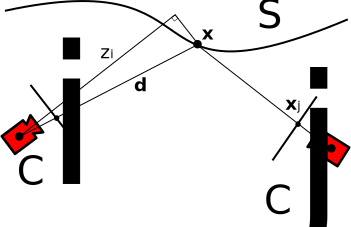
\includegraphics[width=0.5\textwidth]{./img/ch-incr-dens/cameproj}
\label{fig:cameraproj}
\caption{Variables involved in the photometric refinement process}.
\end{figure}

The equation of the gradient functional becomes:
\begin{equation}
  DE(\mathit{S})_v = \sum_i v_i \int_{\mathit{S}} \phi_i(x) \nabla E(x) \textrm{d}x.
\end{equation}

The discrete version of this gradient computed for a single vertex of the mesh becomes:
\begin{equation}
  \frac{\textrm{d}E(\mathit{S})}{\textrm{d}X_i} =  \int_{\mathit{S}} \phi_i(x) \nabla E(x) \textrm{d}x.
\end{equation}

In our case we need to compute the gradient of the energy defined in equation \eqref{eq:energy_photo}:
\begin{equation}
  \nabla E_{\textrm{photo}} = \nabla (\sum_{i,j} err_{ij}(x)) = \sum_{i,j} \nabla err_{ij}(x).
\end{equation}
As in \cite{pons2007multi} we suppose the point $x$ projects in points $x^i = \Pi_i(x) \in I_i$ and  $x^j = \Pi_j(x) \in I_j$, then, the vector $\mathbf{d}_i$ goes from camera $i$ to point $x$, $z_i$ is the depth of $x$ in camera $i$, final $\mathbf{N}$ is the normal at $x$ pointing outward the surface $\mathit{S}$. 
Therefore, with the change of variable $\textrm{d}x_i = -\mathbf{N}^T \mathbf{d}_i \textrm{d}x/z_i^3$:
\begin{equation}
  \nabla \mathit{M}_{ij}(x) = -\mathbf{N} \left( \partial_2 err_{I_i, I_{ij}^{\mathit{S}}}(x_i) DI_j(x_j) D\Pi_j(x)\frac{\mathbf{d}_i}{z_i^3}\right) = - f_{ij}(x_i) \mathbf{N}/z_i^3.
\end{equation}
where operator $D$ represents the derivative and $\partial_2 err_{I_i, I_{ij}^{\mathit{S}}}(x_i)$ is the derivative of $err_{ij}(x)$ with respect to the second image.


We then are able to rewrite the discrete gradient:
\begin{equation}
  \frac{\textrm{d}E(\mathit{S})}{\textrm{d}X_i} =  - \int_{\mathit{S}} \phi_i(x) \sum_{i,j} \mathit{M}_{ij}(x) \textrm{d}x 
\end{equation}

\begin{equation}
  =  - \sum_{i,j} \int_{\mathit{S}} \phi_i(x)  f_{ij}(x_i)  \mathbf{N}/z_i^3 \textrm{d}x 
\end{equation}
\begin{equation}
  =  - \sum_{i,j} \int_{\mathit{S}} \phi_i(x)  f_{ij}(x_i)  \mathbf{N}/z_i^3 \frac{z_i^3}{\mathbf{N}^T \mathbf{d}_i }\mathbf{N} \textrm{d}x_i
\end{equation}

\begin{equation}
\label{eq:final}
  =  - \sum_{i,j} \int_{\mathit{\Omega_{i,j}}} \phi_i(x)  f_{ij}(x_i)  \mathbf{N}/z_i^3 \frac{z_i^3}{\mathbf{N}^T \mathbf{d}_i }\mathbf{N} \textrm{d}x_i
\end{equation}

where $\Omega_{i,j}$ represents the surface region that induces the projection of image $I_j$ into the image $I_i$.

On the other hand, we minimize the energy $E_{\textrm{smooth}}$ as in \cite{vu_et_al_2012} by means of the Laplace-Beltrami operator approximated with the umbrella operator \cite{wardetzky2007discrete}.


% \begin{figure}[t]
% \centering
% 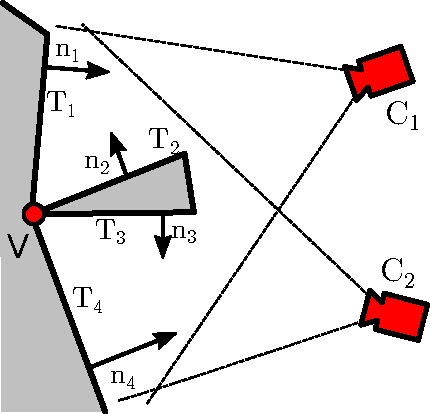
\includegraphics[width=0.5\textwidth]{./img/ch-incr-dens/whymanifold}
% \label{fig:whymanifold}
% \caption{Simple illustration of an in-coherency induced in the photomentric refinement step by the non-manifoldness of vertex $v$}.
% \end{figure}


\subsection{Why manifoldness?}
\label{subsec:why}
In Section \ref{sec:incremental_manifold} we focus our efforts to keep the manifold property valid.
After the description of the surface evolution method, we are now able to give a more in-depth about manifoldness and the importance of this property.


\begin{figure}[t]
\centering
\begin{tabular}{ccc}
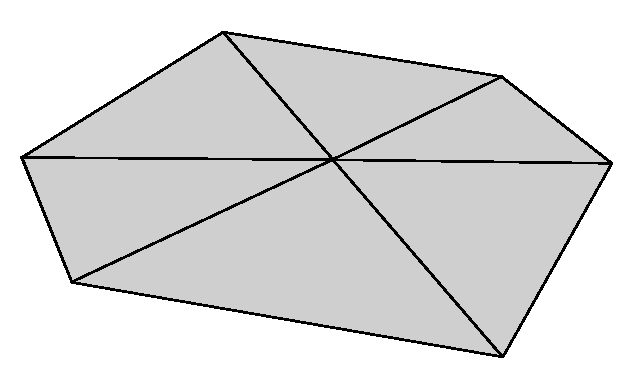
\includegraphics[width=0.28\columnwidth]{img/ch-incr-dens/manifold}&
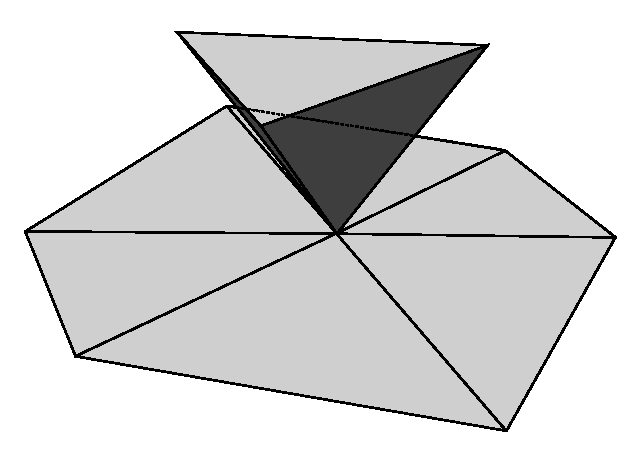
\includegraphics[width=0.28\columnwidth]{img/ch-incr-dens/notmanifold1}&
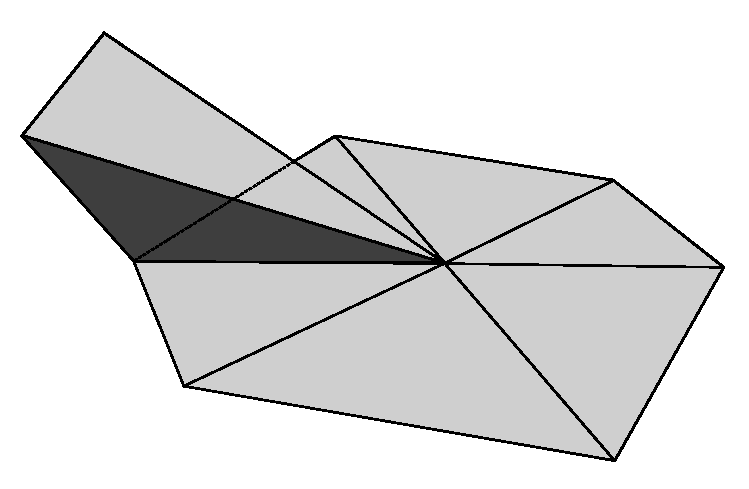
\includegraphics[width=0.28\columnwidth]{img/ch-incr-dens/notmanifold2}\\
(a)&(b)&(c)
\end{tabular}
\caption{The manifold property: the vertex $V$ in (a) is regular ($ABCDEF$ is a closed path without cycles), while in (b) and (c) the vertex $V$ is not regular since, in the former case the path $ABCDEFGHI$ is not closed, and in the latter $ABCDEFGHF$ has two cycles.}
\label{fig:vertexManifold}
\end{figure}


Let recall that the manifold property holds if and only if the neighborhood of each surface point is homeomorphic to a disk. 
So a mesh, which is a discrete surface, is manifold if and only if each vertex $v$ is \emph{regular}, i.e., if and only if the edges opposite to $v$ form a closed path without loops  \cite{litvinov_lhuillier_13}. 
We show in Figure \ref{fig:vertexManifold} (a) one example of a regular vertex and in Figure \ref{fig:vertexManifold}(b) and \ref{fig:vertexManifold}(c) two cases where the vertices are not regular and thus they break the manifold property.
involves the estimation of a mesh which usually partitions the 3D Delaunay Triangulation of a set of sparse points between two sets: free space and matter.
In this case, the sources of non-manifoldness can be induced by tetrahedra intersecting at a vertex, and by tetrahedra with a common edge (non-manifold edge). 
In both cases the non-manifoldness can be fixed, in principle, by cloning and offsetting the vertex of intersection, but two big drawbacks arise: this process would invalidate the Delaunay property, that we need to keep valid in an incremental setting, and, since many non-manifold vertices are generated, rearranging the triangulation and the visibility information for each non-manifold point becomes inefficient. For these two reasons we need a different approach to enforce the manifoldness.
%%resolution

The surface evolution method described such far, collects the contributions of the gradient from the image, for each vertex of the mesh \eqref{eq:final}. Therefore non-manifold meshes, would lead to non-consistent contribution to the computation. See for example Fig. \ref{fig:whymanifold}, Equation \eqref{eq:final} for the vertex $V$ sum up the gradient contribution carried by the triangles $T_1$, $T_2$, $T_3$ and $T_4$; these contribution contains contradictory information , since normals $n_1$, $n_2$, $n_3$ and $n_4$ have very different directions.

\begin{figure}[t]
\centering
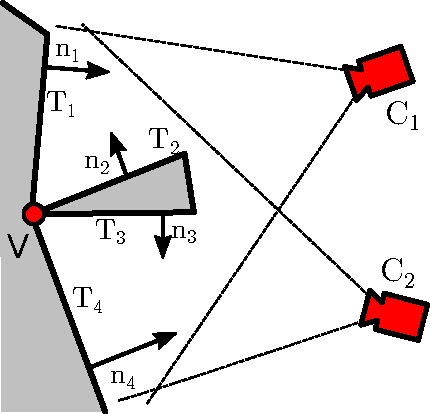
\includegraphics[width=0.5\textwidth]{./img/ch-incr-dens/whymanifold}
\label{fig:whymanifold}
\caption{Simple illustration of an in-coherency induced in the photomentric refinement step by the non-manifoldness of vertex $v$}.
\end{figure}


\subsection{Manifold-preserving Mesh Stitching}
\label{sec:Mesh_merging}
In the proposed system we need to merge the manifold mesh reconstructed incrementally with the mesh after the refinement.
In this paper we propose a new merging approach: the existing methods such as \cite{turk1994zippered} and \cite{VuPhD011},  deal with meshes with similar resolution and significant overlap. 
In particular  Vu   \cite{VuPhD011} merges together two mesh refined; he re-triangulate the overlapping areas and stitches the borders through graph cut-algorithm over the 3D Constrained Delauna triangulation of the border edges.
These approach only merges similar resolution and good overlapping meshes, it fixes a-posteriori the non-manifoldnesses and, the surface evolution refinement is not directly applied to the stitched areas.

In our case, in order to incrementally reconstruct and refine the whole mesh we need to attach the missing part of the scene as soon as the rough reconstruction is available. Therefore we propose a new approach to merge the two meshes which have very different resolutions and a significant overlap is rarely available. Moreover after the merging step we refine both the new region of the scene and the neighboring old part so that it accomodates its vertices more coherently.


The main idea is to keep as facet as possible from the refined manifold mesh: we find the two non intersecting boundary of the two meshes such that in the next step we join them an we the manifold property holds the merged mesh.

Let $\mathit{M}_{0..t}^{\text{rec}}$ and  $\mathit{M}_{0..t}^{\text{opt}}$ be the new manifold and the refined mesh which we aim at merging, e.g., blue and green meshes in Fig. \ref{fig:mesh_merging}(a).


First, we erase all the facets  $f^{\text{rec}} \in \mathit{M}_{0..t}^{\text{rec}}$ close to $f^{\text{opt}} \in \mathit{M}_{0..t}^{\text{opt}}$, i.e., all the $f^{\text{rec}}$ whose bounding boxes intersect at least one of the bounding boxes of the facets $f^{\text{opt}}$ (in Fig. \ref{fig:mesh_merging}(b) and Fig. \ref{fig:mesh_merging}(c))).
Once the facets have been removed, $\mathit{M}_{0..t}^{\text{rec}}$ becomes a set of connected components (meshes); we keep the biggest one, whose boundary is the ordered set of edges $\mathit{b}^{\text{rec}} = \{b_1^{\text{rec}}, \dots,  b_k^{\text{rec}}\}$.

%Then, we define a second ordered set of edges $\mathit{b}^{\text{opt}} = \{b_1^{\text{opt}}, \dots,  b_k^{\text{opt}}\}$ belonging to  $\mathit{M}_{0..t}^{\text{opt}}$ such that the facets we will add to join the two edges, will likely preserve the manifoldness.
We define the set of facets $\hat{f}^{\text{opt}}$ near to $\mathit{b}^{\text{rec}}$, as the intersection among  $k^{bound}$ times the bounding boxes around the facets adjacent to  $\mathit{b}^{\text{rec}}$ and the bounding boxes of $f^{\text{opt}}$  (green faces and their adjacent edges in Fig. \ref{fig:mesh_merging}(d)).
Now, let  $v_{\text{start}}^{\text{opt}}$ and $v_{\text{end}}^{\text{opt}}$ be the two vertices nearest to the extremity of  $\mathit{b}^{\text{rec}}$. 
We define $\mathit{b}^{\text{opt}}$ as the path from $v_{\text{start}}^{\text{opt}}$ to $v_{\text{end}}^{\text{opt}}$ among the edges of the facets in $\hat{f}^{\text{opt}}$ which minimizes the energy:
\begin{equation}
  E_{\text{path}}(b^{\text{opt}}) = \angle (\overrightarrow{n}_b^{\text{opt}},\overrightarrow{n}^{\text{opt-rec}})
\end{equation}
where $\overrightarrow{n}_b^{\text{opt}}$ is the normal of the facet belonging to $\mathit{b}^{\text{opt}}$ and adjacent to  $b^{\text{opt}}$; and
$\overrightarrow{n}^{\text{opt-rec}}$ is the normal of the facet defined by the two vertices $A$ and $B$, extremity of current edge ${b}^{\text{opt}}$ and the nearest vertex in the border $\mathit{b}^{\text{rec}}$ to the vertices $A$ and $B$.
We minimize $E_{\text{path}}$ with the Dijkstra algorithm  (Fig. \ref{fig:mesh_merging}(e)).

Finally we connect the corresponding extremities of the two borders $\mathit{b}^{\text{rec}}$ and $\mathit{b}^{\text{opt}}$, and we create the joining facets by filling the polyline hole with the algorithm of \cite{liepa2003filling}  (Fig. \ref{fig:mesh_merging}(f)).

%FLEXYbilit

\begin{figure}[t]
\begin{tabular}{ccc}
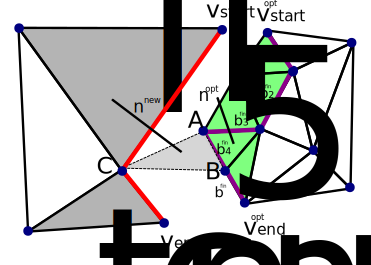
\includegraphics[width=0.3\textwidth]{./img/ch-incr-dens/meshmerge01}&
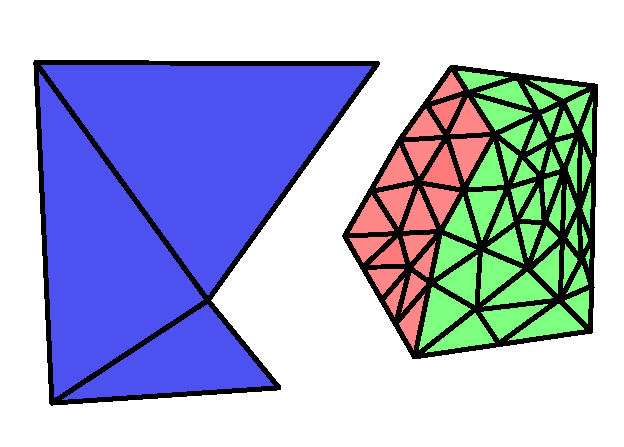
\includegraphics[width=0.3\textwidth]{./img/ch-incr-dens/meshmerge03}&
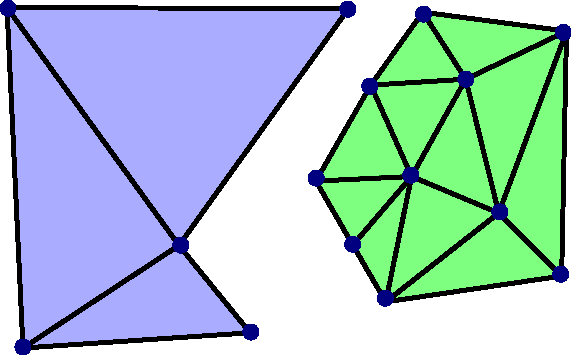
\includegraphics[width=0.3\textwidth]{./img/ch-incr-dens/meshmerge04}\\
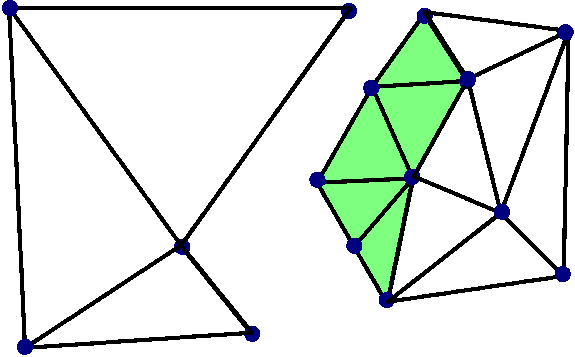
\includegraphics[width=0.3\textwidth]{./img/ch-incr-dens/meshmerge07}&
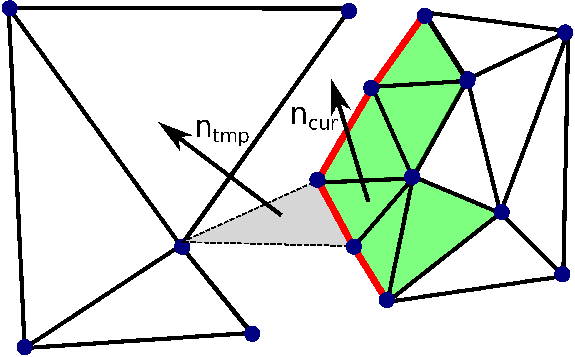
\includegraphics[width=0.3\textwidth]{./img/ch-incr-dens/meshmerge09}&
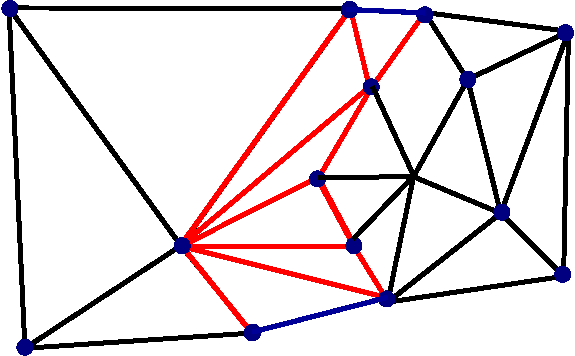
\includegraphics[width=0.3\textwidth]{./img/ch-incr-dens/meshmerge11}
\end{tabular}
\label{fig:mesh_merging}
\caption{Mesh merging steps}
\end{figure}



\section{Experimental Evaluation}
\label{sec:exp}

\section{Conclusion and Future Works}
\label{sec:concl}
In this paper we propose a novel incremental accurate 3D reconstruction algorithm which builds a continuous manifold mesh by leveraging on the novel incremental reconstruction algorithms from sparse point cloud and state-of-the-art multi-view stereo techniques. 
We propose a novel mesh merging algorithm that joints incrementally multi-resolute meshes. 
Our algorithm is able to reconstruct both small objects and large-scenes thanks to the mesh representation and the underlying Delaunay Triangulation which is self adaptive with respect to the scene.

As a future work we aim at integrating the new mesh sweeping algorithm proposed in  \cite{romanoni16} which would provide an intermediate step between the manifold reconstruction and the photometric refinement and would improve the convergence.





